%! Author = gonca
%! Date = 15 Jan 2024

\documentclass{article}
\usepackage[portuguese]{babel}
\usepackage[utf8]{inputenc}
\usepackage{graphicx}
\usepackage{hyperref}
\usepackage{url}
\usepackage{booktabs}

\title{UÉvora\\IAA - MEI 2023/2024\\Projecto de Avaliação\\\textbf{Análise de Dados de Vinhos Portugueses}}
\author{\textbf{Gonçalo Candeias Amaro}\\Número 56870}
\date{15 Jan 2024}

\begin{document}

    \maketitle

    \begin{abstract}
        Este relatório apresenta uma análise de vinhos portugueses ``Vinho Verde'' e modelos de machine learning para previsão de qualidade e teor alcoólico, bem como a distinção entre vinhos tintos e brancos.
    \end{abstract}


    \section{Introdução}
    Introdução ao projeto e aos conjuntos de dados.


    \section{Análise Exploratória de Dados}

    \subsection{Visão Geral Rápida}
    Esta subsecção apresenta uma visão geral inicial dos conjuntos de dados.

    Foi possível observar que os conjuntos de dados possuem 12 colunas cada (acidez fixa, acidez volátil, ácido cítrico, açúcar residual, cloretos, dióxido de enxofre livre, dióxido de enxofre total, densidade, pH, sulfatos, álcool, qualidade).

    As colunas de atributos são todas numéricas. Os valores são todos float64 ou int32.

    Foi feito uma inspeção rápida onde se encontrou que havia \textit{outliers} em algumas colunas, e três valores nulos no conjunto de dados de vinhos brancos e vermelhos.

    Como a imagem abaixo mostra, no vinho branco, na acidez fixa, existem um caso desses \textit{outliers}:

    \begin{figure}
        \centering
        \begin{minipage}{0.90\textwidth}
            \centering
            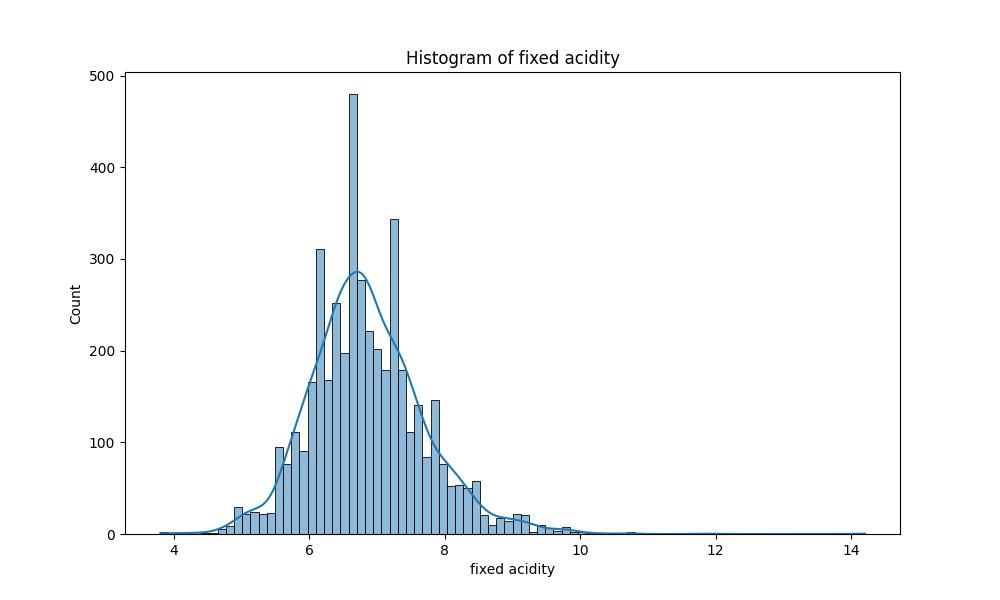
\includegraphics[width=\textwidth]{../out/graphs/eda/white_fixed_acidity_histogram.jpg}
            \caption{Outliers na acidez fixa do vinho branco.}
            \label{fig:white_fixed_acidity}
        \end{minipage}
    \end{figure}

    \subsection{Valores Nulos ou Ausentes}
    Seguidamente, tratamos da presença de valores nulos ou ausentes nos conjuntos de dados, convertendo os tipos de dados para os tipos mais adequados e substitui valores nulos ou ausentes por \texttt{pd.NA}.

    Com isso, foi possível observar que os conjuntos de dados não possuem mais valores nulos ou ausentes. O valor \texttt{pd.NA} já é um valor nulo, mas é tratado de forma diferente pelo pandas. Com isto em mente, podemos dizer que os conjuntos de dados não possuem mais valores nulos ou ausentes (os quais possam dar problemas na análise).

    \subsection{Detecção de \textit{outliers} e Tratamento}
    Para identificar e tratar \textit{outliers}, utilizamos o \texttt{winsorize} da biblioteca \texttt{scipy.stats} para substituir os \textit{outliers} por valores próximos aos limites do intervalo de confiança.

    \texttt{Winsorize} é uma função que recebe um array e retorna um array com os \textit{outliers} substituídos. O parâmetro \texttt{limits} é um tuple que define os limites do intervalo de confiança. Neste caso, os limites são 0.05 e 0.95, o que significa que os valores abaixo do percentile 5 e acima do percentile 95 serão substituídos.

    O tratamento dos tipos de dados já está incluído na função \texttt{parse\_and\_clean}, que força a conversão de todos os valores para o tipo correto.

    \subsection{Normalização dos Dados}
    Para normalizar os dados, utilizamos o \texttt{RobustScaler}. Em que os dados são normalizados usando a seguinte fórmula:

    \begin{equation}
        X_{scaled} = \frac{X - Q_1(X)}{Q_3(X) - Q_1(X)}
    \end{equation}

    Onde $Q_1(X)$ é o primeiro quartil e $Q_3(X)$ é o terceiro quartil.
    Este metodo por si já trata os \textit{outliers}, pois o \texttt{RobustScaler} é um método robusto, no entanto, foi utilizado o método \texttt{handle\_\textit{outliers}} para garantir que os \textit{outliers} fossem tratados antes da normalização.

    É tambem resistentes a \textit{pd.NA}.

    \subsection{Fusão e Exportação dos Dados Tratados}
    Para terminar esta secção, fundimos os conjuntos de dados de vinhos brancos e vinhos tintos e exportamos o conjunto de dados tratado para um ficheiro CSV.


    \section{Análise Exploratória de Dados}

    Ainda no mesmo script, foram feitas algumas análises exploratórias de dados. A seguir, apresentamos os resultados.

    \subsection{Distribuição de Atributos}
    A distribuição de atributos foi analisada usando um metodo chamado \texttt{eda} que recebe um conjunto de dados e o tipo de vinho (tinto ou branco) e gera um histograma para cada coluna do conjunto de dados.

    Este faz output do método \texttt{describe} em que retorna um resumo estatístico dos dados. Seguido do método \texttt{histplot} da biblioteca \texttt{seaborn} gera um histograma para cada coluna do conjunto de dados.

    Aqui o eda foi chamado duas vezes, uma para cada conjunto de dados. Os resultados foram salvos em \texttt{out/graphs}.

    \subsection{Correlação entre Atributos}
    A correlação entre atributos foi analisada usando o método \texttt{corr} da biblioteca \texttt{pandas} retorna uma matriz de correlação entre os atributos. O método \texttt{heatmap} da biblioteca \texttt{seaborn} gera um mapa de calor para a matriz de correlação.

    O gráfico de correlação gerado para os vinhos tintos é apresentado na Figura~\ref{fig:corr_red} e o gráfico de correlação gerado para os vinhos brancos é apresentado na Figura~\ref{fig:corr_white}.

    \begin{figure}
        \centering
        \begin{minipage}{0.45\textwidth}
            \centering
            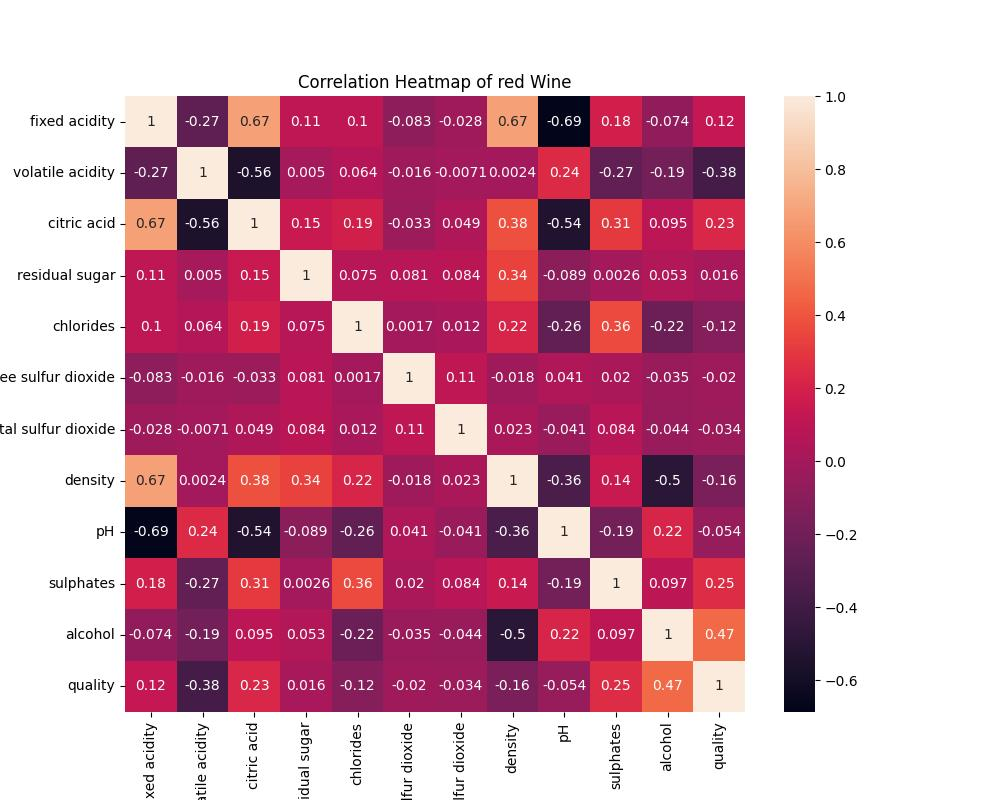
\includegraphics[width=\textwidth]{../out/graphs/red_correlation.jpg}
            \caption{Mapa de calor da correlação entre os atributos dos vinhos tintos.}
            \label{fig:corr_red}
        \end{minipage}
        \hfill
        \begin{minipage}{0.45\textwidth}
            \centering
            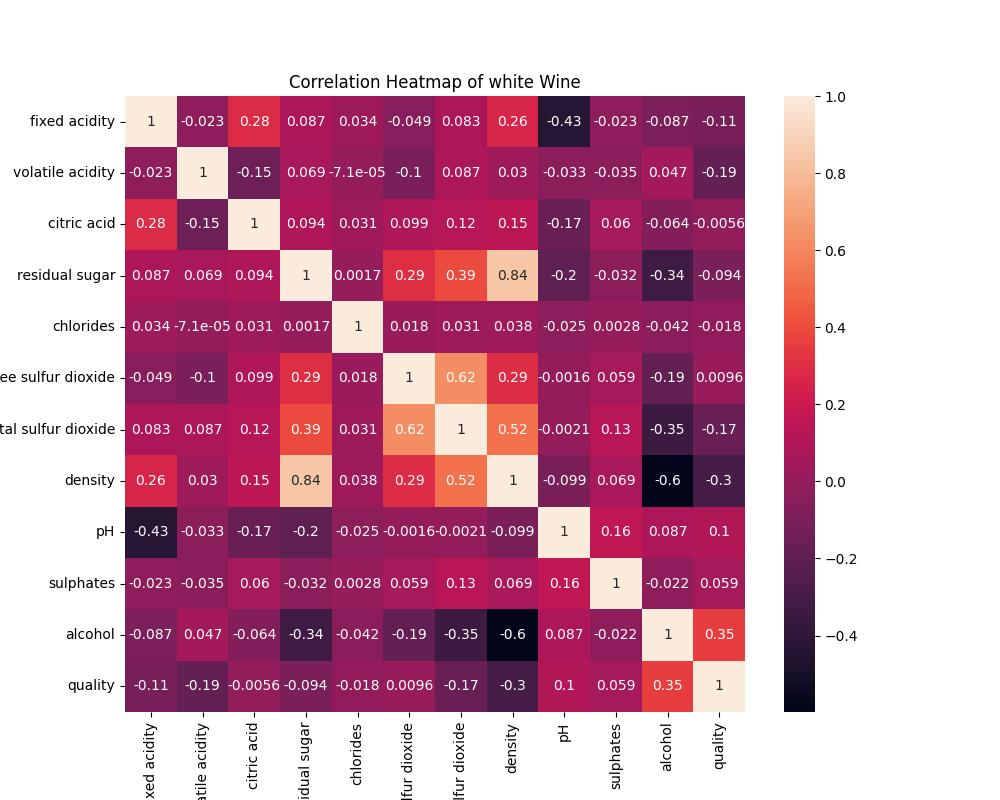
\includegraphics[width=\textwidth]{../out/graphs/white_correlation.jpg}
            \caption{Mapa de calor da correlação entre os atributos dos vinhos brancos.}
            \label{fig:corr_white}
        \end{minipage}
    \end{figure}

    Como podemos observar, os atributos mais correlacionados com a qualidade são o álcool e a acidez volátil. Os atributos mais correlacionados com o álcool são a densidade e o açúcar residual. Os atributos mais correlacionados com a acidez volátil são o ácido cítrico e o pH.


    \section{Tarefa de Regressão}

    Com esta tarefa, pretendemos prever o nível de álcool dos vinhos através dos outros atributos com modelos de regressão.

    \subsection{Previsão de nível de álcool}
    Para prever o nível de álcool, utilizamos os seguintes modelos:

    \begin{enumerate}
        \item Regressão Linear
        \item Regressão de Floresta Aleatória
    \end{enumerate}

    Os quais foram implementados usando o ficheiro: \texttt{src/task1.py}.

    Com estes modelos, obtivemos os seguintes resultados:

    \begin{table}[ht]
        \centering
        \begin{tabular}{@{}lll@{}}
            \toprule
            Modelo                          & MSE  & R2 Score \\ \midrule
            Regressão Linear                & 0.11 & 0.71     \\
            Regressão de Floresta Aleatória & 0.05 & 0.87     \\ \bottomrule
        \end{tabular}
        \caption{Resultados da tarefa de regressão.}
        \label{tab:task1_results}
    \end{table}

    Com base nos resultados apresentados na Tabela \ref{tab:task1_results}, podemos concluir que o modelo de regressão de floresta aleatória é o mais adequado para prever o nível de álcool. Este modelo obteve um MSE de 0.05 e um R2 Score de 0.87, enquanto que o modelo de regressão linear obteve um MSE de 0.11 e um R2 Score de 0.71.

    Não só sendo melhor na previsão como tambem nos proporciona a a oportunidade de analisar a importancia de cada atributo para a previsão.

    \begin{figure}[ht]
        \centering
        \begin{minipage}{0.90\textwidth}
            \centering
            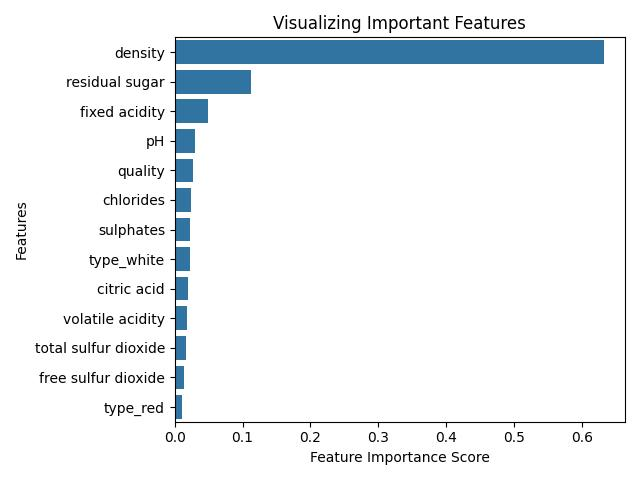
\includegraphics[width=\textwidth]{../out/graphs/feature_importance.jpg}
            \caption{Importância dos atributos para a previsão do nível de álcool.}
            \label{fig:task1_feature_importance}
        \end{minipage}
    \end{figure}

    Como podemos observar na Figura \ref{fig:task1_feature_importance}, os atributos mais importantes para a previsão do nível de álcool são a densidade, o açúcar residual e o pH.


    \section{Tarefa de Classificação}

    Com esta tarefa, pretendemos prever o tipo de vinho (tinto ou branco) através dos outros atributos com modelos de classificação.

    \subsection{Previsão do tipo de vinho}

    Para prever o tipo de vinho, utilizamos os seguintes modelos:

    \begin{enumerate}
        \item Regressão Logística
        \item Floresta Aleatória
    \end{enumerate}

    Os quais foram implementados usando o ficheiro: \texttt{src/task2.py}.

    om estes modelos, obtivemos os seguintes resultados:

    \begin{table}[ht]
        \centering
        \begin{tabular}{@{}lllll@{}}
            \toprule
            Modelo              & Accuracy & F1 Score & Precisão & Recall \\ \midrule
            Regressão Logística & 0.77     & 0.33     & 0.73     & 0.21   \\
            Floresta Aleatória  & 0.97     & 0.94     & 1.0      & 0.90   \\ \bottomrule
        \end{tabular}
        \caption{Resultados da tarefa de classificação.}
        \label{tab:task2_results}
    \end{table}

    \begin{figure}[ht]
        \centering
        \begin{minipage}{0.45\textwidth}
            \centering
            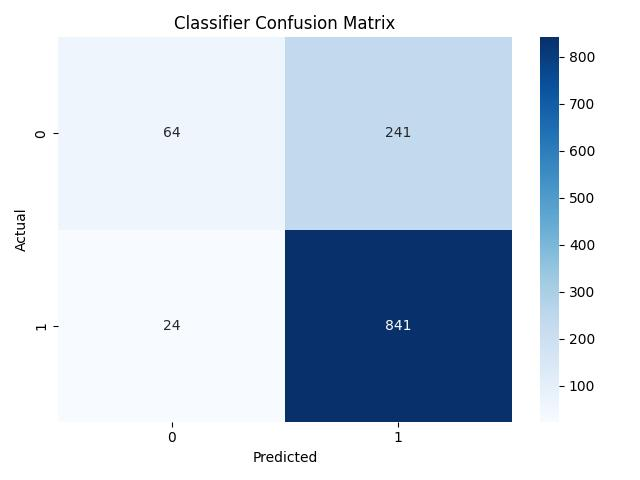
\includegraphics[width=\textwidth]{../out/graphs/task2_log_reg_matrix.jpg}
            \caption{Matriz de confusão para o modelo de floresta aleatória.}
            \label{fig:task2_random_forest_matrix}
        \end{minipage}
        \hfill
        \begin{minipage}{0.45\textwidth}
            \centering
            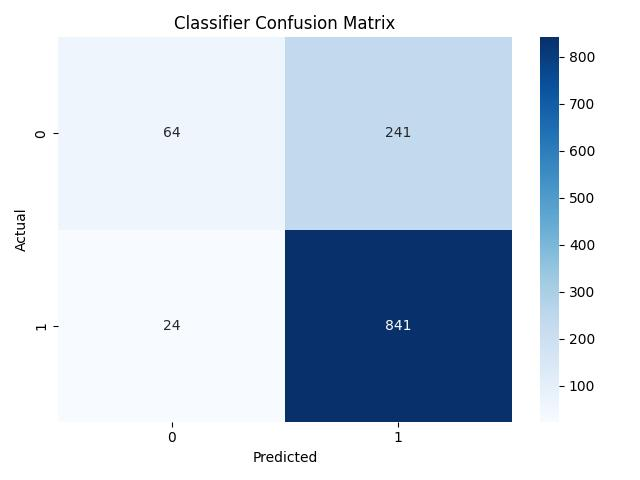
\includegraphics[width=\textwidth]{../out/graphs/task2_log_reg_matrix.jpg}
            \caption{Matriz de confusão para o modelo de regressão logística.}
            \label{fig:task2_log_reg_matrix}
        \end{minipage}
    \end{figure}

    Com base nos resultados apresentados na Tabela~\ref{tab:task2_results}, podemos concluir que o modelo de floresta aleatória é o mais adequado para prever o tipo de vinho. Este modelo obteve uma \textit{accuracy} de 0.97, um F1 Score de 0.94, uma precisão de 1.0 e um \textit{recall} de 0.90, enquanto que o modelo de regressão logística obteve uma \textit{accuracy} de 0.77, um F1 Score de 0.33, uma precisão de 0.73 e um \textit{recall} de 0.21.

    Continuando a moda anterior dos modelos de floresta aleatória serem os melhores para este caso de estudo especifico.

    \begin{figure}
        \centering
        \begin{minipage}{0.90\textwidth}
            \centering
            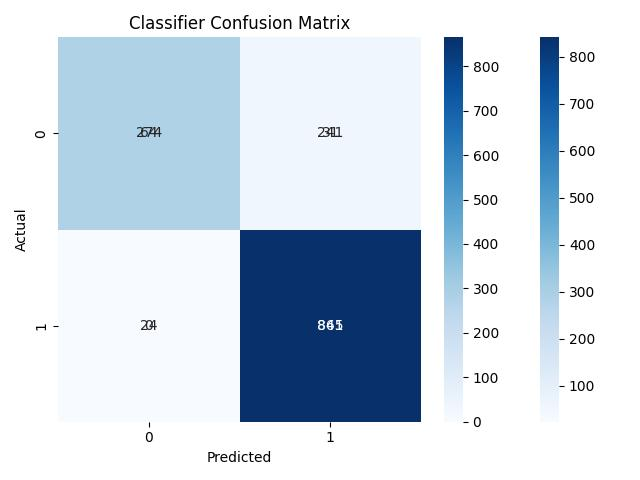
\includegraphics[width=\textwidth]{../out/graphs/task2_rfc_matrix.jpg}
            \caption{Matriz de confusão para o modelo de floresta aleatória.}
            \label{fig:task2_random_forest_matrix}
        \end{minipage}
    \end{figure}


    \section{Tarefa de previsão de qualidade}

    Com esta tarefa, pretendemos prever a qualidade dos vinhos através dos outros atributos com modelos de classificação.

    \subsection{Previsão da qualidade dos vinhos}

    Para prever a qualidade dos vinhos, utilizamos os seguintes modelos:

    \begin{enumerate}
        \item \textit{Gradient Boosting Regressor}
        \item \textit{K-Nearest Neighbors Regressor}
        \item \textit{Linear Regression}
        \item \textit{Random Forest Regressor}
        \item \textit{Support Vector Regressor}
    \end{enumerate}

    Os quais foram implementados usando o ficheiro: \texttt{src/task3.py}.

    Com estes modelos, obtivemos os seguintes resultados:

    \begin{table}[ht]
        \centering
        \begin{tabular}{@{}llll@{}}
            \toprule
            Modelo                                 & MSE  & R2 Score & MAE  \\ \midrule
            \textit{Gradient Boosting Regressor}   & 0.33 & 0.37     & 0.47 \\
            \textit{K-Nearest Neighbors Regressor} & 0.35 & 0.32     & 0.46 \\
            \textit{Linear Regression}             & 0.37 & 0.27     & 0.50 \\
            \textit{Random Forest Regressor}       & 0.26 & 0.51     & 0.39 \\
            \textit{Support Vector Regressor}      & 0.32 & 0.37     & 0.44 \\ \bottomrule
        \end{tabular}
        \caption{Resultados da tarefa de previsão de qualidade.}
        \label{tab:task3_results}
    \end{table}

    Com base nos resultados apresentados na Tabela~\ref{tab:task3_results}, podemos concluir que o modelo de floresta aleatória é o mais adequado para prever a qualidade dos vinhos. Este modelo obteve um MSE de 0.26, um R2 Score de 0.51 e um MAE de 0.39, enquanto que os outros modelos obtiveram um MSE entre 0.32 e 0.37, um R2 Score entre 0.27 e 0.37 e um MAE entre 0.44 e 0.50.

    A \textit{trend} continua, o modelo de floresta aleatória é o melhor para este caso de estudo.


    \section{Conclusão}
    Foi efetuada uma análise exploratória de dados e foram implementados modelos de machine learning para previsão de qualidade e teor alcoólico, bem como a distinção entre vinhos tintos e brancos. Os modelos de floresta aleatória foram os mais adequados para prever o teor alcoólico, o tipo de vinho e a qualidade dos vinhos.

    \newpage

    \begin{thebibliography}{9}

        \bibitem{winequality}
        Towards Data Science.
        \url{https://towardsdatascience.com/wine-quality-prediction-using-machine-learning-9c5cbc8b148b}.

        \bibitem{randomforests}
        DataCamp.
        \url{https://www.datacamp.com/community/tutorials/random-forests-classifier-python}.

        \bibitem{svm}
        DataCamp.
        \url{https://www.datacamp.com/community/tutorials/svm-classification-scikit-learn-python}.

        \bibitem{knn}
        DataCamp.
        \url{https://www.datacamp.com/community/tutorials/k-nearest-neighbor-classification-scikit-learn}.

        \bibitem{logisticregression}
        DataCamp.
        \url{https://www.datacamp.com/community/tutorials/understanding-logistic-regression-python}.

        \bibitem{chatopenai}
        ChatGPT Queries. (Debug python outputs)
        \url{https://chat.openai.com/}.

    \end{thebibliography}

\end{document}
